% questions.tex —— 2006 年·普通高等学校招生考试·福建卷理科 · 题目内容片段（无答案）
% 由 tools/generate_projects.py 依来源总账自 2006/2006_数学真题_福建理_试题.md 生成，勿手改（改源 MD 后重跑）


\begin{gktip}
\textbf{来源边界}：据固定 PDF 第1—2页转录，印刷页码288—289。来源清单中的 ready 只代表固定文件通过格式检查，不是发布者、版次或官方身份认证。固定 PDF 仅见题面，未见答案、解析或评分标准。
\textbf{转录说明}：按原页保留题意，不依推测补写分值或答案。Q7“对于平面 $\alpha$ 和共面的直线 $m$、$n$”按字面照录；Q16、Q18、Q20 图稿依据固定 PDF 重绘，仅表达图中标注和拓扑，不补充题设条件。文字层中的平行符号、根式、指数和乘积关系均按页图复核。
\end{gktip}

\gkpart{一、选择题}

\begin{question}
\gkti{1}设 $a,b,c,d\in\mathbb R$，则复数 $(a+bi)(c+di)$ 为实数的充要条件是\mbox{（　　）}

（A）$ad-bc=0$　　（B）$ac-bd=0$　　（C）$ac+bd=0$　　（D）$ad+bc=0$

\end{question}
\begin{question}
\gkti{2}在等差数列 $\{a_n\}$ 中，已知 $a_1=2$，$a_2+a_3=13$，则 $a_4+a_5+a_6$ 等于\mbox{（　　）}

（A）$40$　　（B）$42$　　（C）$43$　　（D）$45$

\end{question}
\begin{question}
\gkti{3}已知 $\alpha\in\left(\dfrac{\pi}{2},\pi\right)$，$\sin\alpha=\dfrac35$，则 $\tan\left(\alpha+\dfrac\pi4\right)$ 等于\mbox{（　　）}

（A）$\dfrac17$　　（B）$7$　　（C）$-\dfrac17$　　（D）$-7$

\end{question}
\begin{question}
\gkti{4}已知全集 $U=\mathbb R$，且 $A=\{x\mid |x-1|>2\}$，$B=\{x\mid x^2-6x+8<0\}$，则 $(C_U A)\cap B$ 等于\mbox{（　　）}

（A）$[-1,4)$　　（B）$(2,3)$　　（C）$(2,3]$　　（D）$(-1,4)$

\end{question}
\begin{question}
\gkti{5}已知正方体外接球的体积是 $\dfrac{32}{3}\pi$，那么正方体的棱长等于\mbox{（　　）}

（A）$2\sqrt2$　　（B）$\dfrac{2\sqrt3}{3}$　　（C）$\dfrac{4\sqrt2}{3}$　　（D）$\dfrac{4\sqrt3}{3}$

\end{question}
\begin{question}
\gkti{6}在一个口袋中装有 $5$ 个白球和 $3$ 个黑球，这些球除颜色外完全相同，从中摸出 $3$ 个球，至少摸到 $2$ 个黑球的概率等于\mbox{（　　）}

（A）$\dfrac27$　　（B）$\dfrac38$　　（C）$\dfrac37$　　（D）$\dfrac9{28}$

\end{question}
\begin{question}
\gkti{7}对于平面 $\alpha$ 和共面的直线 $m$、$n$，下列命题中真命题是\mbox{（　　）}

（A）若 $m\perp\alpha$，$m\perp n$，则 $n\parallel\alpha$

（B）若 $m\parallel\alpha$，$n\parallel\alpha$，则 $m\parallel n$

（C）若 $m\subset\alpha$，$n\parallel\alpha$，则 $m\parallel n$

（D）若 $m$、$n$ 与 $\alpha$ 所成的角相等，则 $m\parallel n$

\end{question}
\begin{question}
\gkti{8}函数 $y=\log_2\dfrac{x}{x-1}\ (x>1)$ 的反函数是\mbox{（　　）}

（A）$y=\dfrac{2^x}{2^x-1}\ (x>0)$　　（B）$y=\dfrac{2^x}{2^x-1}\ (x<0)$

（C）$y=\dfrac{2^x-1}{2^x}\ (x>0)$　　（D）$y=\dfrac{2^x-1}{2^x}\ (x<0)$

\end{question}
\begin{question}
\gkti{9}已知函数 $f(x)=2\sin\omega x\ (\omega>0)$ 在区间 $\left[-\dfrac\pi3,\dfrac\pi4\right]$ 上的最小值是 $-2$，则 $\omega$ 的最小值等于\mbox{（　　）}

（A）$\dfrac23$　　（B）$\dfrac32$　　（C）$2$　　（D）$3$

\end{question}
\begin{question}
\gkti{10}已知双曲线 $\dfrac{x^2}{a^2}-\dfrac{y^2}{b^2}=1\ (a>0,\ b>0)$ 的右焦点为 $F$，若过点 $F$ 且倾斜角为 $60^\circ$ 的直线与双曲线的右支有且只有一个交点，则此双曲线离心率的取值范围是\mbox{（　　）}

（A）$(1,2]$　　（B）$(1,2)$　　（C）$[2,+\infty)$　　（D）$(2,+\infty)$

\end{question}
\begin{question}
\gkti{11}已知 $|\overrightarrow{OA}|=1$，$|\overrightarrow{OB}|=\sqrt3$，$\overrightarrow{OA}\cdot\overrightarrow{OB}=0$，点 $C$ 在 $\angle AOB$ 内，且 $\angle AOC=30^\circ$。设 $\overrightarrow{OC}=m\overrightarrow{OA}+n\overrightarrow{OB}\ (m,n\in\mathbb R)$，则 $\dfrac mn$ 等于\mbox{（　　）}

（A）$\dfrac13$　　（B）$3$　　（C）$\dfrac{\sqrt3}{3}$　　（D）$\sqrt3$

\end{question}
\begin{question}
\gkti{12}对于直角坐标平面内的任意两点 $A(x_1,y_1)$、$B(x_2,y_2)$，定义它们之间的一种“距离”：$\lVert AB\rVert=|x_2-x_1|+|y_2-y_1|$。给出下列三个命题：

① 若点 $C$ 在线段 $AB$ 上，则 $\lVert AC\rVert+\lVert CB\rVert=\lVert AB\rVert$；

② 在 $\triangle ABC$ 中，若 $\angle C=90^\circ$，则 $\lVert AC\rVert^2+\lVert CB\rVert^2=\lVert AB\rVert^2$；

③ 在 $\triangle ABC$ 中，$\lVert AC\rVert+\lVert CB\rVert>\lVert AB\rVert$。

其中真命题的个数为\mbox{（　　）}

（A）$1$　　（B）$2$　　（C）$3$　　（D）$4$

\end{question}
\gkpart{二、填空题}

\begin{question}
\gkti{13}$\left(x^2-\dfrac{1}{x}\right)^5$ 展开式中 $x^4$ 的系数是\gkblank{}。（用数字作答）

\end{question}
\begin{question}
\gkti{14}已知直线 $x-y-1=0$ 与抛物线 $y=ax^2$ 相切，则 $a=$\gkblank{}。

\end{question}
\begin{question}
\gkti{15}一个均匀小正方体的六个面中，三个面上标以数 $0$，两个面上标以数 $1$，一个面上标以数 $2$。将这个小正方体抛掷 $2$ 次，则向上的数之积的数学期望是\gkblank{}。

\Needspace{0.4\textheight}
\end{question}
\begin{question}
\gkti{16}如图，连结 $\triangle ABC$ 的各边中点得到一个新的 $\triangle A_1B_1C_1$，又连结 $\triangle A_1B_1C_1$ 的各边中点得到一个新的 $\triangle A_2B_2C_2$，如此无限继续下去，得到一系列三角形：$\triangle ABC$，$\triangle A_1B_1C_1$，$\triangle A_2B_2C_2$，$\cdots$，这一系列三角形趋向于一个点 $M$。已知 $A(0,0)$，$B(3,0)$，$C(2,2)$，则点 $M$ 的坐标是\gkblank{}。
\nopagebreak[4]
\begin{center}% Source: 2006 Fujian science candidate PDF, source ID
% src-ab0f2729ee4a24495e653b44c14438b4130f8b38b11362bf84251f3595a09d27,
% SHA-256 50d17546b94af82fb2cee653942752914cd387fe72792d74ffa5f75e7a301d83,
% page 1, printed page 288, Q16. Schematic reconstruction; not a measurement drawing.
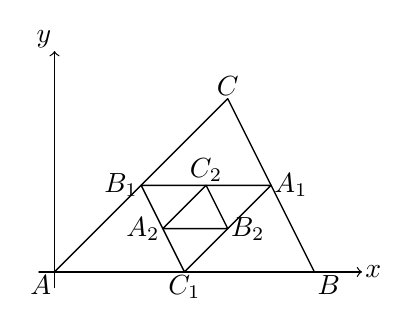
\begin{tikzpicture}[x=1.1cm,y=1.1cm,line cap=round,line join=round]
  \coordinate (A)  at (0,0);
  \coordinate (B)  at (3,0);
  \coordinate (C)  at (2,2);
  \coordinate (A1) at (2.5,1);
  \coordinate (B1) at (1,1);
  \coordinate (C1) at (1.5,0);
  \coordinate (A2) at (1.25,0.5);
  \coordinate (B2) at (2,0.5);
  \coordinate (C2) at (1.75,1);

  % Coordinate axes shown in the source diagram.
  \draw[->,line width=0.45pt] (0,-0.18) -- (0,2.55);
  \draw[->,line width=0.45pt] (-0.18,0) -- (3.55,0);

  % Original triangle and the first two midpoint triangles.
  \draw[line width=0.5pt] (A)--(B)--(C)--cycle;
  \draw[line width=0.5pt] (A1)--(B1)--(C1)--cycle;
  \draw[line width=0.5pt] (A2)--(B2)--(C2)--cycle;

  \node[below left,inner sep=1pt]  at (A)  {$A$};
  \node[below right,inner sep=1pt] at (B)  {$B$};
  \node[above,inner sep=1pt]       at (C)  {$C$};
  \node[right,inner sep=1pt]       at (A1) {$A_1$};
  \node[left,inner sep=1pt]        at (B1) {$B_1$};
  \node[below,inner sep=1pt]       at (C1) {$C_1$};
  \node[left,inner sep=1pt]        at (A2) {$A_2$};
  \node[right,inner sep=1pt]       at (B2) {$B_2$};
  \node[above,inner sep=1pt]       at (C2) {$C_2$};
  \node[above left,inner sep=1pt]  at (0,2.55) {$y$};
  \node[right,inner sep=1pt]       at (3.55,0) {$x$};
\end{tikzpicture}
\end{center}
\nopagebreak[4]
\end{question}
\gkpart{三、解答题}

\begin{question}
\gkti{17}已知函数
\nopagebreak[4]
\[
f(x)=\sin^2 x+\sqrt{3}\sin x\cos x+2\cos^2 x,\quad x\in\mathbb{R}.
\]

（1） 求函数 $f(x)$ 的最小正周期和单调增区间；

（2） 函数 $f(x)$ 的图象可以由函数 $y=\sin 2x\ (x\in\mathbb{R})$ 的图象经过怎样的变换得到？

\Needspace{0.4\textheight}
\end{question}
\begin{question}
\gkti{18}如图，四面体 $ABCD$ 中，$O$、$E$ 分别是 $BD$、$BC$ 的中点，$CA=CB=CD=BD=2$，$AB=AD=\sqrt{2}$。

（1） 求证：$AO\perp$ 平面 $BCD$；

（2） 求异面直线 $AB$ 与 $CD$ 所成角的大小；

（3） 求点 $E$ 到平面 $ACD$ 的距离。
\nopagebreak[4]
\begin{center}% Source: 2006 Fujian science candidate PDF, source ID
% src-ab0f2729ee4a24495e653b44c14438b4130f8b38b11362bf84251f3595a09d27,
% SHA-256 50d17546b94af82fb2cee653942752914cd387fe72792d74ffa5f75e7a301d83,
% page 1, printed page 288, Q18. Schematic positions only; lengths and angles are not encoded.
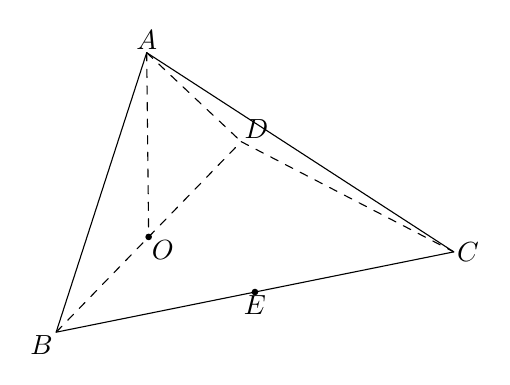
\begin{tikzpicture}[line cap=round,line join=round]
  \coordinate (A) at (1.15,3.55);
  \coordinate (B) at (0,0);
  \coordinate (C) at (5.05,1.02);
  \coordinate (D) at (2.35,2.42);
  \coordinate (O) at (1.175,1.21); % midpoint of BD
  \coordinate (E) at (2.525,0.51); % midpoint of BC

  % Visible and hidden edges of the tetrahedron.
  \draw (A)--(B)--(C)--cycle;
  \draw[dashed] (A)--(D);
  \draw[dashed] (B)--(D);
  \draw[dashed] (D)--(C);
  \draw[dashed] (A)--(O);

  \fill (O) circle (1.2pt);
  \fill (E) circle (1.2pt);
  \node[above,inner sep=1pt]       at (A) {$A$};
  \node[below left,inner sep=1pt]  at (B) {$B$};
  \node[right,inner sep=1pt]       at (C) {$C$};
  \node[above right,inner sep=1pt] at (D) {$D$};
  \node[below right,inner sep=1pt] at (O) {$O$};
  \node[below,inner sep=1pt]       at (E) {$E$};
\end{tikzpicture}
\end{center}
\nopagebreak[4]
\end{question}
\begin{question}
\gkti{19}统计表明，某种型号的汽车在匀速行驶中每小时的耗油量 $y$（升）关于行驶速度 $x$（千米/小时）的函数解析式可以表示为：
\nopagebreak[4]
\[
y=\frac{1}{128000}x^3-\frac{3}{80}x+8\quad(0<x\le120).
\]
已知甲、乙两地相距 $100$ 千米。

（1） 当汽车以 $40$ 千米/小时的速度匀速行驶时，从甲地到乙地要耗油多少升？

（2） 当汽车以多大的速度匀速行驶时，从甲地到乙地耗油最少？最少为多少升？

\Needspace{0.4\textheight}
\end{question}
\begin{question}
\gkti{20}已知椭圆 $\dfrac{x^2}{2}+y^2=1$ 的左焦点为 $F$，$O$ 为坐标原点。

（1） 求过点 $O$、$F$，并且与椭圆的左准线 $l$ 相切的圆的方程；

（2） 设过点 $F$ 且不与坐标轴垂直的直线交椭圆于 $A$、$B$ 两点，线段 $AB$ 的垂直平分线与 $x$ 轴交于点 $G$，求点 $G$ 横坐标的取值范围。
\nopagebreak[4]
\begin{center}% Source: 2006 Fujian science candidate PDF, source ID
% src-ab0f2729ee4a24495e653b44c14438b4130f8b38b11362bf84251f3595a09d27,
% SHA-256 50d17546b94af82fb2cee653942752914cd387fe72792d74ffa5f75e7a301d83,
% page 2, printed page 289, Q20. Chord direction and all placements are schematic.
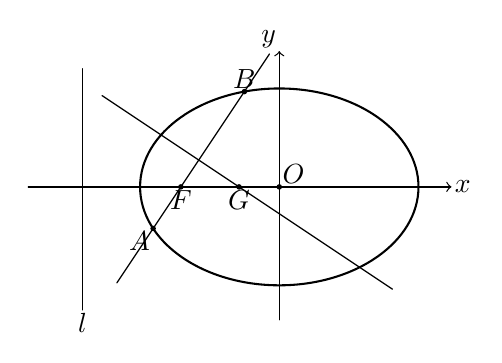
\begin{tikzpicture}[x=1.25cm,y=1.25cm,line cap=round,line join=round]
  \pgfmathsetmacro{\xA}{(-9-sqrt(26))/11}
  \pgfmathsetmacro{\yA}{3*(2-sqrt(26))/22}
  \pgfmathsetmacro{\xB}{(-9+sqrt(26))/11}
  \pgfmathsetmacro{\yB}{3*(2+sqrt(26))/22}
  \coordinate (A) at (\xA,\yA);
  \coordinate (B) at (\xB,\yB);
  \coordinate (F) at (-1,0);
  \coordinate (O) at (0,0);
  \coordinate (G) at (-9/22,0);
  \coordinate (M) at (-9/11,3/11); % midpoint of AB

  % Axes and left directrix l: x=-2.
  \draw[->,line width=0.45pt] (-2.55,0) -- (1.75,0);
  \draw[->,line width=0.45pt] (0,-1.35) -- (0,1.38);
  \draw[line width=0.45pt] (-2,-1.25) -- (-2,1.2);

  % Ellipse x^2/2+y^2=1.
  \draw[line width=0.75pt] (O) ellipse [x radius=1.4142,y radius=1];

  % One schematic secant through F and its perpendicular bisector.
  % The chosen slope only locates the drawing; it is not given data.
  \draw[line width=0.45pt] (-1.65,-0.975) -- (-0.1,1.35);
  \draw[line width=0.45pt] (-1.8,0.9273) -- (1.15,-1.0394);

  \fill (A) circle (1pt);
  \fill (B) circle (1pt);
  \fill (F) circle (1pt);
  \fill (O) circle (1pt);
  \fill (G) circle (1pt);

  \node[below left,inner sep=1pt]  at (A) {$A$};
  \node[above,inner sep=1pt]       at (B) {$B$};
  \node[below,inner sep=1pt]       at (F) {$F$};
  \node[above right,inner sep=1pt] at (O) {$O$};
  \node[below,inner sep=1pt]       at (G) {$G$};
  \node[above left,inner sep=1pt]  at (0,1.38) {$y$};
  \node[right,inner sep=1pt]       at (1.75,0) {$x$};
  \node[below,inner sep=1pt]       at (-2,-1.25) {$l$};
\end{tikzpicture}
\end{center}
\nopagebreak[4]
\end{question}
\begin{question}
\gkti{21}已知函数 $f(x)=-x^2+8x$，$g(x)=6\ln x+m$。

（1） 求 $f(x)$ 在区间 $[t,t+1]$ 上的最大值 $h(t)$；

（2） 是否存在实数 $m$，使得 $y=f(x)$ 的图象与 $y=g(x)$ 的图象有且只有三个不同的交点？若存在，求出 $m$ 的取值范围；若不存在，说明理由。

\end{question}
\begin{question}
\gkti{22}已知数列 $\{a_n\}$ 满足 $a_1=1$，$a_{n+1}=2a_n+1\ (n\in\mathbb{N}^*)$。

（1） 求数列 $\{a_n\}$ 的通项公式；

\Needspace{5\baselineskip}
（2） 若数列 $\{b_n\}$ 满足
\nopagebreak[4]
\[
4^{b_1-1}4^{b_2-1}4^{b_3-1}\cdots4^{b_n-1}=(a_n+1)^{b_n}\quad(n\in\mathbb{N}^*),
\]
证明 $\{b_n\}$ 是等差数列；

\Needspace{5\baselineskip}
（3） 证明：
\nopagebreak[4]
\[
\frac{n}{2}-\frac{1}{3}<\frac{a_1}{a_2}+\frac{a_2}{a_3}+\cdots+\frac{a_n}{a_{n+1}}<\frac{n}{2}\quad(n\in\mathbb{N}^*).
\]

\end{question}